%%
%% Design Approach
%%
%% This file should be edited by user
%%

%%%%%%%%%%%%%%%%%%%%%%%%%%%%%%%%%%%%%%%%%%%%%%%%%%%%%%%%%%%%%%%%%%%%%%%%%%%%%%%%
\chapter{\emph{simavr} Internals} \label{chapter:simavr}
%%%%%%%%%%%%%%%%%%%%%%%%%%%%%%%%%%%%%%%%%%%%%%%%%%%%%%%%%%%%%%%%%%%%%%%%%%%%%%%%

It is necessary to understand \emph{simavr}'s internals before going on to discuss
\emph{qsimavr}'s design.

\emph{simavr} is a small cross-platform \ac{AVR} simulator written with simplicity and
hackability in mind. It is supported on Linux and OS X, but should run on any
platform with avr-libc support.

In the following sections, we will take a tour through \emph{simavr} internals\footnote{
Most, if not all of the code examined in this chapter is taken directly from \emph{simavr}.}.
Without further delay, let's jump right in and walk through a short demo.


%%%%%%%%%%%%%%%%%%%%%%%%%%%%%%%%%%%%%%%%%%%%%%%%%%%%%%%%%%%%%%%%%%%%%%%%%%%%%%%%
\section{\emph{simavr} Example Walkthrough} \label{section:simavr_example_walkthrough}
%%%%%%%%%%%%%%%%%%%%%%%%%%%%%%%%%%%%%%%%%%%%%%%%%%%%%%%%%%%%%%%%%%%%%%%%%%%%%%%%

The following program is taken from the board\_i2ctest \emph{simavr} example. Minor
modifications have been made to focus on the essential section. Error handling
is mostly omitted in favor of readability.

\begin{lstlisting}
#include <stdlib.h>
#include <stdio.h>
#include <libgen.h>
#include <pthread.h>

#include "sim_avr.h"
#include "avr_twi.h"
#include "sim_elf.h"
#include "sim_gdb.h"
#include "sim_vcd_file.h"
#include "i2c_eeprom.h"
\end{lstlisting}

The actual simulation of the external \ac{EEPROM} component is located in
i2c\_eeprom.h. We will take a look at the implementation later on.

\begin{lstlisting}
avr_t * avr = NULL;
avr_vcd_t vcd_file;

i2c_eeprom_t ee;
\end{lstlisting}

avr is the main data structure. It encapsulates the entire state of the
core simulation, including register, \ac{SRAM} and flash contents, the \ac{CPU} state, the
current cycle count, callbacks for various tasks, pending interrupts, and more.

\lstinline|vcd_file| represents the file target for the \emph{value change dump} module. It
is used to dump the level changes of desired pins (or \acp{IRQ} in general) into a
file which can be subsequently viewed using utilities such as \emph{gtkwave}.

\lstinline|ee| contains the internal state of the simulated external \ac{EEPROM}.

\begin{lstlisting}
int main(int argc, char *argv[])
{
    elf_firmware_t f;
    elf_read_firmware("atmega1280_i2ctest.axf", &f);
\end{lstlisting}

The firmware is loaded from the specified file. Note that exactly the same file
can be executed on the \ac{AVR} hardware without changes. \ac{MCU} and frequency
information have been embedded into the binary and are therefore available in
\lstinline|elf_firmware_t|.

\begin{lstlisting}
    avr = avr_make_mcu_by_name(f.mmcu);
    avr_init(avr);
    avr_load_firmware(avr, &f);
\end{lstlisting}

The \lstinline|avr_t| instance is then constructed from the core file of the
specified \ac{MCU} and initialized. \lstinline|avr_load_firmware| copies the
firmware into program memory.

\begin{lstlisting}
    i2c_eeprom_init(avr, &ee, 0xa0, 0xfe, NULL, 1024);
    i2c_eeprom_attach(avr, &ee, AVR_IOCTL_TWI_GETIRQ(0));
\end{lstlisting}

\lstinline|AVR_IOCTL_TWI_GETIRQ| is a macro to retrieve the internal \ac{IRQ} of the \ac{TWI}
simulation. \acp{IRQ} are the main method of communication between \emph{simavr} and
external components and are also used liberally throughout \emph{simavr} internals.
Similar macros exist for other important \ac{AVR} parts such as the \ac{ADC}, \ac{IO} ports,
timers, etc.

\begin{lstlisting}
    avr->gdb_port = 1234;
    avr->state = cpu_Stopped;
    avr_gdb_init(avr);
\end{lstlisting}

This section sets up \emph{simavr}'s \ac{GDB} infrastructure to listen on port 1234. The
\ac{CPU} is stopped to allow \ac{GDB} to attach before execution begins.

\begin{lstlisting}
    avr_vcd_init(avr, "gtkwave_output.vcd", &vcd_file, 100000 /* usec */);
    avr_vcd_add_signal(
        &vcd_file,
        avr_io_getirq(avr, AVR_IOCTL_TWI_GETIRQ(0), TWI_IRQ_STATUS),
        8 /* bits */,
        "TWSR");
\end{lstlisting}

Next, a value change dump output is configured to track changes to the
\lstinline|TWI_IRQ_STATUS| \ac{IRQ}. The file may then be viewed using the \emph{gtkwave}
application.

\begin{lstlisting}
    int state = cpu_Running;
    while ((state != cpu_Done) && (state != cpu_Crashed))
        state = avr_run(avr);

    return 0;
}
\end{lstlisting}

Finally, we have reached the simple main loop. Each iteration executes one
instruction, handles any pending interrupts and cycle timers, and sleeps if
possible. As soon as execution completes or crashes, simulation stops and we
exit the program.

We will now examine the relevant parts of the \lstinline|i2c_eeprom| implementation.
Details have been omitted and only communication with the \lstinline|avr_t| instance are
shown.

\begin{lstlisting}
static const char * _ee_irq_names[2] = {
		[TWI_IRQ_MISO] = "8>eeprom.out",
		[TWI_IRQ_MOSI] = "32<eeprom.in",
};

void
i2c_eeprom_init(
		struct avr_t * avr,
		i2c_eeprom_t * p,
		uint8_t addr,
		uint8_t mask,
		uint8_t * data,
		size_t size)
{

    /* [...] */

	p->irq = avr_alloc_irq(&avr->irq_pool, 0, 2, _ee_irq_names);
	avr_irq_register_notify(p->irq + TWI_IRQ_MOSI, i2c_eeprom_in_hook, p);

    /* [...] */
}
\end{lstlisting}

First, the \ac{EEPROM} allocates its own private \acp{IRQ}. The \ac{EEPROM} implementation
does not know or care to which \emph{simavr} \acp{IRQ} they will be attached. It then
attaches a callback function (\lstinline|i2c_eeprom_in_hook|) to the \ac{MOSI} \ac{IRQ}. This
function will be called whenever a value is written to the \ac{IRQ}. The pointer to
the \ac{EEPROM} state p is passed to each of these callback function calls.

\begin{lstlisting}
void
i2c_eeprom_attach(
		struct avr_t * avr,
		i2c_eeprom_t * p,
		uint32_t i2c_irq_base )
{
	avr_connect_irq(
		p->irq + TWI_IRQ_MISO,
		avr_io_getirq(avr, i2c_irq_base, TWI_IRQ_MISO));
	avr_connect_irq(
		avr_io_getirq(avr, i2c_irq_base, TWI_IRQ_MOSI),
		p->irq + TWI_IRQ_MOSI );
}
\end{lstlisting}

The private \acp{IRQ} are then attached to \emph{simavr}'s internal \acp{IRQ}. This is called
chaining - all messages raised are forwarded to all chained \acp{IRQ}.

\begin{lstlisting}
static void
i2c_eeprom_in_hook(
		struct avr_irq_t * irq,
		uint32_t value,
		void * param)
{
	i2c_eeprom_t * p = (i2c_eeprom_t*)param;

    /* [...] */

    avr_raise_irq(p->irq + TWI_IRQ_MISO,
            avr_twi_irq_msg(TWI_COND_ACK, p->selected, 1));

    /* [...] */
}
\end{lstlisting}

Finally, we've reached the \ac{IRQ} callback function. It is responsible for
simulating communications between \emph{simavr} (acting as the \ac{TWI} master) and the
\ac{EEPROM} (as the \ac{TWI} slave). The \ac{EEPROM} state which was previously passed to
\lstinline|avr_irq_register_notify| is contained in the \lstinline|param| variable and cast back to
an \lstinline|i2c_eeprom_t| pointer for further use.

Outgoing messages are sent by raising the internal \ac{IRQ}. This message is then
forwarded to all chained \acp{IRQ}.


%%%%%%%%%%%%%%%%%%%%%%%%%%%%%%%%%%%%%%%%%%%%%%%%%%%%%%%%%%%%%%%%%%%%%%%%%%%%%%%%
\section{Main Loop} \label{section:mainloop}
%%%%%%%%%%%%%%%%%%%%%%%%%%%%%%%%%%%%%%%%%%%%%%%%%%%%%%%%%%%%%%%%%%%%%%%%%%%%%%%%

We will now take a closer look at the main loop implementation. Each call to
\lstinline|avr_run| triggers the function stored in the run member of the \lstinline|avr_t| structure
(\lstinline|avr->run|\footnote{Whenever \lstinline|avr| is mentioned in a code
section, it is assumed to be the main \lstinline|avr_t| struct.}).
The two standard implementations are \lstinline|avr_callback_run_raw| and
\lstinline|avr_callback_run_gdb|, located in sim\_avr.c. The essence of both function is
identical; since \lstinline|avr_callback_run_gdb| contains additional logic for \ac{GDB}
handling (network protocol, stepping), we will examine it further and point out
any differences to the the raw version. Several comments and irrelevant code
sections have been removed.

\begin{lstlisting}
void avr_callback_run_gdb(avr_t * avr)
{
    avr_gdb_processor(avr, avr->state == cpu_Stopped);

    if (avr->state == cpu_Stopped)
        return ;

    int step = avr->state == cpu_Step;
    if (step)
        avr->state = cpu_Running;
\end{lstlisting}

This initial section is \ac{GDB} specific. \lstinline|avr_gdb_processor| is responsible for
handling \ac{GDB} network communication. It also checks if execution has reached a
breakpoint or the end of a step and stops the \ac{CPU} if it did.

If \ac{GDB} has transmitted a step command, we need to save the state during the
main section of the loop (the \ac{CPU} ``runs'' for one instruction) and restore to
the ``StepDone'' state at on completion.

\begin{lstlisting}
    avr_flashaddr_t new_pc = avr->pc;

    if (avr->state == cpu_Running) {
        new_pc = avr_run_one(avr);
    }
\end{lstlisting}

We have now reached the actual execution of the current instruction. If the \ac{CPU}
is currently running, \lstinline|avr_run_one| decodes the instruction located in flash memory
(\lstinline|avr->flash|) and triggers all necessary actions. This can include setting the \ac{CPU}
state (SLEEP), updating the status register \ac{SREG}, writing or reading from memory
locations, altering the \ac{PC}, etc \ldots

Finally, the cycle counter (\lstinline|avr->cycle|) is updated and the new
program counter is returned.

\begin{lstlisting}
    if (avr->sreg[S_I] && !avr->i_shadow)
        avr->interrupts.pending_wait++;
    avr->i_shadow = avr->sreg[S_I];
\end{lstlisting}

This section ensures that interrupts are not triggered immediately when
enabling the interrupt flag in the status register, but with an (additional)
delay of one instruction.

\begin{lstlisting}
    avr_cycle_count_t sleep = avr_cycle_timer_process(avr);
    avr->pc = new_pc;
\end{lstlisting}

Next, all due cycle timers are processed. Cycle timers are one of the
most important and heavily used mechanisms in \emph{simavr}. A timer allows scheduling
execution of a callback function once a specific count of execution cycles have
passed, thus simulating events which occur after a specific amount of time has
passed. For example, the \lstinline|avr_timer| module uses cycle timers to schedule timer
interrupts.

The returned estimated sleep time is set to the next pending event cycle (or a
hardcoded limit of 1000 cycles if none exist).

\begin{lstlisting}
    if (avr->state == cpu_Sleeping) {
        if (!avr->sreg[S_I]) {
            avr->state = cpu_Done;
            return;
        }
        avr->sleep(avr, sleep);
        avr->cycle += 1 + sleep;
    }
\end{lstlisting}

If the \ac{CPU} is currently sleeping, the time spent is simulated using the callback
stored in \lstinline|avr->sleep|. In \ac{GDB} mode, the time is used to listen for
\ac{GDB} commands, while the raw version simply calls usleep.

It is worth noting that
we have improved the timing behavior by accumulating requested sleep cycles until
a minimum of 200 usec has been reached. usleep cannot handle lower sleep times
accurately, which caused an unrealistic execution slowdown.

A special case occurs when the \ac{CPU} is sleeping while interrupts are turned off.
In this scenario, there is way of ever waking up. Therefore, execution is halted
gracefully.

\begin{lstlisting}
    if (avr->state == cpu_Running || avr->state == cpu_Sleeping)
        avr_service_interrupts(avr);
\end{lstlisting}

Finally, any immediately pending interrupts are handled. The highest priority
interrupt (this depends solely on the interrupt vector address) is removed from
the pending queue, interrupts are disabled in the status register, and the
program counter is set to the interrupt vector.

If the \ac{CPU} is sleeping, interrupts can be raised by cycle timers.

\begin{lstlisting}
    if (step)
        avr->state = cpu_StepDone;
}
\end{lstlisting}

Wrapping up, if the current loop iteration was a \ac{GDB} step, the state is set
such that the next iteration will inform \ac{GDB} and halt the \ac{CPU}.


%%%%%%%%%%%%%%%%%%%%%%%%%%%%%%%%%%%%%%%%%%%%%%%%%%%%%%%%%%%%%%%%%%%%%%%%%%%%%%%%
\section{Initialization}
%%%%%%%%%%%%%%%%%%%%%%%%%%%%%%%%%%%%%%%%%%%%%%%%%%%%%%%%%%%%%%%%%%%%%%%%%%%%%%%%

%%%%%%%%%%%%%%%%%%%%%%%%%%%%%%%%%%%%%%%%%%%%%%%%%%%%%%%%%%%%%%%%%%%%%%%%%%%%%%%%
\subsection{\lstinline|avr_t| Initialization} \label{subsection:avr_t_initialization}
%%%%%%%%%%%%%%%%%%%%%%%%%%%%%%%%%%%%%%%%%%%%%%%%%%%%%%%%%%%%%%%%%%%%%%%%%%%%%%%%

The \lstinline|avr_t| struct requires some somple initialization before it is
ready to be used by the main loop as discussed in section \ref{section:mainloop}.

\lstinline|avr_make_mcu_by_name| fills in all details specific to an \ac{MCU}. This
includes settings such as memory sizes, register locations, available components,
the default \ac{CPU} frequency, etc \ldots

The \ac{MCU} definitions are located in the simavr/cores subdirectory of the \emph{simavr}
source tree and are compiled conditionally depending on the the local avr-libc
support. A complete list of locally supported cores is printed by running \emph{simavr}
without any arguments.

On successful completion, it returns a pointer to the \lstinline|avr_t| struct.

If \ac{GDB} support is desired, \lstinline|avr->gdb_port| must be set, and
\lstinline|avr_gdb_init| must be called to create the required data structures,
set the \lstinline|avr->run| and \lstinline|avr->sleep| callbacks, and listen
on the specified port. It is also recommended to initially stop the cpu
(\lstinline|avr->state = cpu_Stopped|) to delay program execution until it
is started manually by \ac{GDB}.

Further settings can now be applied manually (typical candidates are logging and
tracing levels).

%%%%%%%%%%%%%%%%%%%%%%%%%%%%%%%%%%%%%%%%%%%%%%%%%%%%%%%%%%%%%%%%%%%%%%%%%%%%%%%%
\subsection{Firmware}
%%%%%%%%%%%%%%%%%%%%%%%%%%%%%%%%%%%%%%%%%%%%%%%%%%%%%%%%%%%%%%%%%%%%%%%%%%%%%%%%

We now have a fully initialized \lstinline|avr_t| struct and are ready to load
code. This is accomplished using \lstinline|avr_read_firmware|, which uses
elfutils to decode the \ac{ELF} file and read it into an \lstinline|elf_firmware_t|
struct and \lstinline|avr_load_firmware| to load its contents into the
\lstinline|avr_t| struct.

Besides loading the program code into \lstinline|avr->flash| (and \ac{EEPROM} contents
into \lstinline|avr->eeprom|, if available), there are several useful extended
features which can be embedded directly into the \ac{ELF} file.

The target \ac{MCU}, frequency and voltages can be specified in the \ac{ELF} file by using the
\lstinline|AVR_MCU| and \lstinline|AVR_MCU_VOLTAGES| macros provided by
avr\_mcu\_section.h:

\begin{lstlisting}
#include "avr_mcu_section.h"
AVR_MCU(16000000 /* Hz */, "atmega1280");
AVR_MCU_VOLTAGES(3300 /* milliVolt */, 3300 /* milliVolt */, 3300 /* milliVolt */);
\end{lstlisting}

\ac{VCD} traces can be set up automatically. The following code will create an 8-bit
trace on the UDR0 register, and a trace masked to display only the UDRE0 bit of
the UCSR0A register.

\begin{lstlisting}
const struct avr_mmcu_vcd_trace_t _mytrace[]  _MMCU_ = {
    { AVR_MCU_VCD_SYMBOL("UDR0"), .what = (void*)&UDR0, },
    { AVR_MCU_VCD_SYMBOL("UDRE0"), .mask = (1 << UDRE0), .what = (void*)&UCSR0A, },
};
\end{lstlisting}

Several predefined commands can be sent from the firmware to \emph{simavr} during program execution.
At the time of writing, these include starting and stopping \ac{VCD} traces, and putting
UART0 into loopback mode. An otherwise unused register must be specified
to listen for command requests. During execution, writing a command to this
register will trigger the associated action within \emph{simavr}.

\begin{lstlisting}
AVR_MCU_SIMAVR_COMMAND(&GPIOR0);

int main() {
    /* [...] */
    GPIOR0 = SIMAVR_CMD_\ac{VCD}_START_TRACE;
    /* [...] */
}
\end{lstlisting}

Likewise, a register can be specified for use as a debugging output. All bytes
written to this register will be output to the console.

\begin{lstlisting}
AVR_MCU_SIMAVR_CONSOLE(&GPIOR0);

int main() {
    /* [...] */
    const char *s = "Hello World\r";
    for (const char *t = s; *t; t++)
        GPIOR0 = *t;
    /* [...] */
}
\end{lstlisting}

Usually, UART0 is used for this purpose. The simplest debug output can be achieved
by binding \lstinline|stdout| to \lstinline|UART0| as described by the avr-libc
documentation \cite{libc}, and then using \lstinline|printf| and similar functions.
This alternate console output is provided in case using UART0 is not possible or desired.



%%%%%%%%%%%%%%%%%%%%%%%%%%%%%%%%%%%%%%%%%%%%%%%%%%%%%%%%%%%%%%%%%%%%%%%%%%%%%%%%
\section{Instruction Processing}
%%%%%%%%%%%%%%%%%%%%%%%%%%%%%%%%%%%%%%%%%%%%%%%%%%%%%%%%%%%%%%%%%%%%%%%%%%%%%%%%

We have now covered \lstinline|avr_t| initialization, the main loop, and loading
firmware files. But how are instructions actually decoded and executed? Let's
take a look at \lstinline|avr_run_one|, located in sim\_core.

The opcode is reconstructed by retrieving the two bytes located at
\lstinline|avr->flash[avr->pc]|. \lstinline|avr->pc| points to the \ac{LSB}, and
\lstinline|avr->pc + 1| to the \ac{MSB}. Thus, the full opcode is reconstructed with:

\begin{lstlisting}
uint32_t opcode = (avr->flash[avr->pc + 1] << 8) | avr->flash[avr->pc];
\end{lstlisting}

As we have seen, \lstinline|avr->pc| represents the byte address in flash memory.
Therefore, the next instruction is located at \lstinline|avr->pc + 2|. This
default new program counter may still be altered in the course of processing
in case of jumps, branches, calls and larger opcodes such as STS\cite{instructionset}.

Note also that the \ac{AVR} flash addresses are usually represented as word addresses
(\lstinline|avr->pc >> 1|).

Similar to the program counter, the spent cycles are set to a default value of 1.

The instruction and its operands are then extracted from the opcode and processed
in a large switch statement. The instructions themselves can be roughly categorized
into arithmetic and logic instructions, branch instructions, data transfer
instructions, bit and bit-test instructions and \ac{MCU} control instructions.

Processing these will involve a number of typical tasks:

\begin{itemize}
\item Status register modifications

The status register is stored in \lstinline|avr->sreg| as a byte array.
Most instructions alter the \ac{SREG} in some way, and convenience functions such as
\lstinline|get_compare_carry| are used to ease this task. Note that whenever the
firmware reads from \ac{SREG}, it must be reconstructed from \lstinline|avr->sreg|.

\item Reading or writing memory

\lstinline|_avr_set_ram| is used to write bytes to a specific address. Accessing
an \ac{SREG} will trigger a reconstruction similar to what has been discussed above.
\ac{IO} register accesses trigger any connected \ac{IO} callbacks and raise all associated
\acp{IRQ}. If a \ac{GDB} watchpoint has been hit, the \ac{CPU} is stopped and a status report
is sent to \ac{GDB}. Data watchpoint support has been added by the author.

\item Modifying the program counter

Jumps, skips, calls, returns and similar instructions alter the program counter.
This is achieved by simply setting \lstinline|new_pc| to an appropriate value. Care must be
taken to skip 32 bit instructions correctly.

\item Altering \ac{MCU} state

Instructions such as SLEEP and BREAK directly alter the state of the simulation.

\item Stack operations

Pushing and popping the stack involve altering the stack pointer in addition
to the actual memory access. 
\end{itemize}

Upon conclusion, \lstinline|avr->cycle| is updated with the actual instruction
duration, and the new program counter is returned.

%%%%%%%%%%%%%%%%%%%%%%%%%%%%%%%%%%%%%%%%%%%%%%%%%%%%%%%%%%%%%%%%%%%%%%%%%%%%%%%%
\section{Interrupts}
%%%%%%%%%%%%%%%%%%%%%%%%%%%%%%%%%%%%%%%%%%%%%%%%%%%%%%%%%%%%%%%%%%%%%%%%%%%%%%%%

An interrupt is an asynchronous signal which causes the the \ac{CPU} to jump to
the associated \ac{ISR} and continue execution there. In the \ac{AVR} architecture,
the interrupt priority is ordered according to its place in the interrupt
vector table. When an interrupt is serviced, interrupts are disabled globally.

%%%%%%%%%%%%%%%%%%%%%%%%%%%%%%%%%%%%%%%%%%%%%%%%%%%%%%%%%%%%%%%%%%%%%%%%%%%%%%%%
\subsection{Data Structures}
%%%%%%%%%%%%%%%%%%%%%%%%%%%%%%%%%%%%%%%%%%%%%%%%%%%%%%%%%%%%%%%%%%%%%%%%%%%%%%%%

Let's take a look at how interrupts are represented in \emph{simavr}:

\begin{lstlisting}
typedef struct avr_int_vector_t {
    uint8_t         vector;
    avr_regbit_t    enable;
    avr_regbit_t    raised;
    avr_irq_t       irq;
    uint8_t         pending : 1,
                    trace : 1,
                    raise_sticky : 1;
} avr_int_vector_t;
\end{lstlisting}

Each interrupt vector has an \lstinline|avr_int_vector_t|. \lstinline|vector| is
actual vector address, for example \lstinline|INT0_vect|. \lstinline|enable|
and \lstinline|raised| specify the \ac{IO} register index for, respectively, the
interrupt enable flag and the interrupt raised bit (again taking \lstinline|INT0|
as an example, enable would point to the \lstinline|INT0| bit in \lstinline|EIMSK|,
and raised to \lstinline|INTF0| in \lstinline|EIFR|. \lstinline|irq| is raised to
1 when the interrupt is triggered, and to 0 when it is serviced.

Usually, raised flags are cleared automatically upon interrupt servicing. However,
this does not count for all interrupts(notably, \lstinline|TWINT|).
\lstinline|raise_sticky| was introduced by the author to handle this special case.

Interrupt vector definitions are stored in an \lstinline|avr_int_table_t|,
\lstinline|avr->interrupts|.

\begin{lstlisting}
typedef struct  avr_int_table_t {
    avr_int_vector_t * vector[64];
    uint8_t         vector_count;
    uint8_t         pending_wait;
    avr_int_vector_t * pending[64];
    uint8_t         pending_w,
                    pending_r;
} avr_int_table_t, *avr_int_table_p;
\end{lstlisting}

\lstinline|pending_wait| stores the number of cycles to wait before servicing
pending interrupts. This simulates the real interrupt delay that occurs between
raising and servicing, and whenever interrupts are enabled
(and previously disabled).

\lstinline|pending| along with \lstinline|pending_w| and \lstinline|pending_r|
represents a ringbuffer of pending interrupts. Note that servicing an
interrupt removes the one with the highest priority.


%%%%%%%%%%%%%%%%%%%%%%%%%%%%%%%%%%%%%%%%%%%%%%%%%%%%%%%%%%%%%%%%%%%%%%%%%%%%%%%%
\subsection{Raising and Servicing Interrupts}
%%%%%%%%%%%%%%%%%%%%%%%%%%%%%%%%%%%%%%%%%%%%%%%%%%%%%%%%%%%%%%%%%%%%%%%%%%%%%%%%

When an interrupt \lstinline|vector| is raised, \lstinline|vector->pending| is
set, \lstinline|vector| is added to the \lstinline|pending| \ac{FIFO} of
\lstinline|avr->interrupts|, and a non-zero \lstinline|pending_wait| time is
ensured. If the \ac{CPU} is currently sleeping, it is woken up.

As we've already covered in section \ref{section:mainloop}, servicing interrupts is
only attempted if the \ac{CPU} is either running or sleeping. Additionally,
interrupts must be enabled globally in \ac{SREG}, and \lstinline|pending_wait|
(which is decremented on each \lstinline|avr_service_interrupts| call) must have
reached zero. The next pending vector with highest priority is then removed from
the pending ringbuffer and serviced as follows:

\begin{lstlisting}
if (!avr_regbit_get(avr, vector->enable) || !vector->pending) {
    vector->pending = 0;
\end{lstlisting}

If the specific interrupt is masked or has been cleared, no action occurs.

\begin{lstlisting}
} else {
    _avr_push16(avr, avr->pc >> 1);
    avr->sreg[S_I] = 0;
    avr->pc = vector->vector * avr->vector_size;
    avr_clear_interrupt(avr, vector);
}
\end{lstlisting}

Otherwise, the current program counter is pushed onto the stack. This illustrates
the difference between byte addresses (as used in \lstinline|avr->pc|) and
word addresses (as expected by the \ac{AVR} processor).
Interrupts are then disabled by clearing the I bit of the status register, and
the program counter is set to the \ac{ISR} vector. Finally, if
\lstinline|raise_sticky| is 0, the interrupt flag is cleared.

%%%%%%%%%%%%%%%%%%%%%%%%%%%%%%%%%%%%%%%%%%%%%%%%%%%%%%%%%%%%%%%%%%%%%%%%%%%%%%%%
\section{Cycle Timers}
%%%%%%%%%%%%%%%%%%%%%%%%%%%%%%%%%%%%%%%%%%%%%%%%%%%%%%%%%%%%%%%%%%%%%%%%%%%%%%%%

Cycle timers allow scheduling an event after a certain amount of cycles have
passed.

\begin{lstlisting}
typedef avr_cycle_count_t (*avr_cycle_timer_t)(
        struct avr_t * avr,
        avr_cycle_count_t when,
        void * param);

void
avr_cycle_timer_register(
        struct avr_t * avr,
        avr_cycle_count_t when,
        avr_cycle_timer_t timer,
        void * param);
\end{lstlisting}

In \lstinline|avr_cycle_timer_register|,
\lstinline|when| is the minimum count of cycles that must pass until the
\lstinline|timer| callback is executed (\lstinline|param| and \lstinline|when|
are passed back to \lstinline|timer|\footnote{
\emph{qsimavr} exploits \lstinline|param| to implement
callbacks to class instances by passing the \lstinline|this| pointer as
\lstinline|param|.})

Once dispatched, the cycle timer is removed from the list of pending timers. If
it returns a nonzero value, it is readded to occur \emph{at or after that cycle has
been reached}. It is important to realize that it therefore differs from the
\lstinline|when| argument of \lstinline|avr_cycle_timer_register|, which expects
a relative cycle count (in contrast to the absolute cycle count returned by the
callback itself)\footnote{
%
Treating the return value of \lstinline|avr_cycle_timer_t| as an absolute value
and passing the actually scheduled cycle allows for precise handling of recurring
timers without drift. A system based on relative cycle counts could not guarantee
accuracy, because \emph{simavr} does not guarantee cycle timer execution exactly at the
scheduled point in time.
}.

The cycle timer system is used during the main loop to determine sleep durations;
if there are any pending timers, the sleep callback may sleep until the next timer
is scheduled. Otherwise, a default value of 1000 cycles is returned.
Besides achieving a runtime behavior similar to execution on a real \ac{AVR}
processor, sleep is important for lowering \emph{simavr} \ac{CPU} usage whenever possible.

\acp{IRQ} and interrupts caused by external events (for example, a ``touch'' event transmitted
from the simulated touchscreen component) are and can \emph{not} be taken into
account.
This means that scheduled sleep times will always be simulated to completion by
\lstinline|avr->sleep|, even if an external event causing \ac{CPU} wakeup is
triggered immediately after going to sleep.
Given a situation in which the next scheduled timer is many cycles in the future
and the \ac{CPU} is currently sleeping, the simulation will become extremely
unresponsive to external events.

However, in real applications this situation is very unprobable, since
manual events (which cannot be scheduled through cycle timers) occur very rarely,
and most applications will have at least some cycle timers with a short period.

It is worth remembering though, that cycle timers are the preferred and most
accurate method of scheduling interrupts in \emph{simavr}.


%%%%%%%%%%%%%%%%%%%%%%%%%%%%%%%%%%%%%%%%%%%%%%%%%%%%%%%%%%%%%%%%%%%%%%%%%%%%%%%%
\section{\acf{GDB}}
%%%%%%%%%%%%%%%%%%%%%%%%%%%%%%%%%%%%%%%%%%%%%%%%%%%%%%%%%%%%%%%%%%%%%%%%%%%%%%%%

A debugger is incredibly useful during program development. Simple programming mistakes
which can be discovered in minutes using \ac{GDB} can sometimes consume hours
to find without it.

We have covered how to enable \ac{GDB} support in section
\ref{subsection:avr_t_initialization}, and when \ac{GDB} handler methods are
called during the main loop in section \ref{section:mainloop}. In the following,
we will explain further the methods \emph{simavr} employs to communicate with
\ac{GDB} and how breakpoints and data watchpoints are implemented. For
a short guide to debugging \ac{AVR} programs with \ac{GDB}, see section
\ref{section:debugging}

\emph{simavr} has a fully featured implementation of the \ac{GDB} Remote Serial Protocol,
which allows it to communicate with \emph{avr-gdb}. A complete reference of
the protocol can be obtained from the \ac{GDB} manual \cite{gdb}. Essentially,
communication boils down to packets of the format \lstinline|$packet-data#checksum|.
The packet data itself consists of a command and its arguments. The syntax of
all commands supported by \emph{simavr} is as follows:

\begin{Verbatim}[samepage=true]
'?' Indicate the reason the target halted.
'G XX...' Write general registers.
'g' Read general registers.
'p n' Read the value of register n.
'P n...=r...' Write register n with value r.
'm addr,length' Read length bytes of memory starting at address
                addr.
'M addr,length:XX...' Write length bytes of memory starting
                      address addr. XX... is the data.
'c' Continue.
's' Step.
'r' Reset the entire system.
'z type,addr,kind' Delete break and watchpoints.
'Z type,addr,kind' Insert break and watchpoints.
\end{Verbatim}

Many of these commands expect a reply value. This could be a simple as sending
\verb|"OK"| to confirm successful execution, or it could contain the requested
data, such as the reply to the \verb|'m'| command. A single reply can chain
several data fields. For example, whenever a watchpoint is hit, the reply contains
the signal the program received (\lstinline|0x05| represents the ``trap'' signal),
the \ac{SREG}, \ac{SP}, and \ac{PC} values, the type of watchpoint which was hit
(either \verb|"awatch"|, \verb|"watch"|, or \verb|"rwatch"|), and the watchpoint
address.

The packets themselves are received and sent over an \lstinline|AF_INET| socket listening
on the \lstinline|avr->gdb_port|.

Both watchpoints and breakpoints are stored within an \lstinline|avr_gdb_watchpoints_t|
struct in \lstinline|avr->gdb| and are limited to 32 active instances of each.
Breakpoints are set at a particular location in flash memory. Whenever the \ac{PC}
reaches that that point, execution is halted, a status report containing a summary
of current register values is sent, and control is passed to \ac{GDB}. This
range check takes place in \lstinline|avr_gdb_processor|, which is called
first during each iteration of the \lstinline|avr_callback_run_gdb| function
as we have already discussed in section \ref{section:mainloop}.

Watchpoints\footnote{Watchpoint support has been added by the author.}
on the other hand are used to notify the user of accesses to \ac{SRAM}.
\ac{GDB} uses a fixed offset of \lstinline|0x800000| to reference locations in
\ac{SRAM}; this offset must be masked out when receiving \ac{GDB} commands, and
added when sending watchpoint status reports.
Three types of watchpoints exist: Read watchpoints are triggered by data reads,
write watchpoints by writes, and access watchpoints by both. Handling of these
is integrated into the \lstinline|avr_core_watch_write| and
\lstinline|avr_core_watch_read| functions. Whenever applicable watchpoints exist
for a data access, execution is halted, and a status report is sent to \ac{GDB}.

Finally, since program crashes often occur unexpectedly, \emph{simavr} helpfully
provides \ac{GDB} passive mode, which
opens a \ac{GDB} listening socket whenever an exception occurs if the \ac{GDB}
port is specified. It is always a good idea to initialize \lstinline|avr->gdb_port| even
if you have no intention of using \emph{simavr}'s \ac{GDB} features!


%%%%%%%%%%%%%%%%%%%%%%%%%%%%%%%%%%%%%%%%%%%%%%%%%%%%%%%%%%%%%%%%%%%%%%%%%%%%%%%%
\section{\acfp{IRQ}}
%%%%%%%%%%%%%%%%%%%%%%%%%%%%%%%%%%%%%%%%%%%%%%%%%%%%%%%%%%%%%%%%%%%%%%%%%%%%%%%%

The \acf{IRQ}\footnote{
%
Despite the name, \acp{IRQ} have nothing in particular to do with interrupts;
the interrupt system uses \acp{IRQ}, and \acp{IRQ} may trigger interrupts, but
they are not strictly linked to each other. Many \ac{IRQ} usages will not involve
interrupts at all.}
%
subsystem provides the message passing mechanism in \emph{simavr}. Let's begin
by examining the main \ac{IRQ} data structures:

\begin{lstlisting}
typedef struct avr_irq_t {
    struct avr_irq_pool_t * pool;
    const char * name;
    uint32_t            irq;
    uint32_t            value;
    uint8_t             flags;
    struct avr_irq_hook_t * hook;
} avr_irq_t;
\end{lstlisting}

An \ac{IRQ} consists of an associated \ac{IRQ} pool, a name (for debugging
purposes), an ID, its current value, flags, and a list of callback functions.
The ID (\lstinline|irq|) is when a callback function connected to several \acp{IRQ}
needs to determine which specific \ac{IRQ} has been raised.

The semantics of \lstinline|value| are not fixed and are specific to each \ac{IRQ};
for example, \lstinline|ADC_IRQ_ADC0| treats \lstinline|value| as milliVolts,
while \lstinline|IOPORT_IRQ_PIN0| expects it to equal either 1 (high) or 0 (low).
\lstinline|flags| is a bitmask of several options\footnote{
%
\lstinline|IRQ_FLAG_ALLOC| and \lstinline|IRQ_FLAG_INIT| are of internal interest
only and not mentioned further.
%
}.
\lstinline|IRQ_FLAG_NOT| flips
the polarity of the signal (raising an \ac{IRQ} with \lstinline|value| 1 results
in a \lstinline|value| of 0 and vice versa).
Setting \lstinline|IRQ_FLAG_FILTERED| instructs \emph{simavr} to ignore \ac{IRQ}
raises with unchanged values.

\lstinline|hook| contains a linked list of chained \acp{IRQ} and
\lstinline|avr_irq_notify_t| callbacks.

\begin{lstlisting}
typedef void (*avr_irq_notify_t)(
        struct avr_irq_t * irq,
        uint32_t value,
        void * param);

void
avr_irq_register_notify(
        avr_irq_t * irq,
        avr_irq_notify_t notify,
        void * param);
\end{lstlisting}

Callbacks are executed whenever an \ac{IRQ} is raised (and is not filtered).
Chained \acp{IRQ} are raised whenever the \ac{IRQ} they are connected to is raised.

As briefly mentioned in section \ref{section:simavr_example_walkthrough}, module
implementations usually structure communication with the \emph{simavr} core by
allocating their own private \acp{IRQ}, which are then connected to the target
\emph{simavr} \acp{IRQ}. Callbacks are registered on private \acp{IRQ};
likewise, only private \acp{IRQ} are raised. This
ensures maximum flexibility since \ac{IRQ} connections are defined in one single
location. Relevant functions are:

\begin{lstlisting}
avr_irq_t *
avr_alloc_irq(
        avr_irq_pool_t * pool,
        uint32_t base,
        uint32_t count,
        const char ** names /* optional */);

void
avr_irq_register_notify(
        avr_irq_t * irq,
        avr_irq_notify_t notify,
        void * param);

void
avr_connect_irq(
        avr_irq_t * src,
        avr_irq_t * dst);

void
avr_raise_irq(
        avr_irq_t * irq,
        uint32_t value);
\end{lstlisting}


%%%%%%%%%%%%%%%%%%%%%%%%%%%%%%%%%%%%%%%%%%%%%%%%%%%%%%%%%%%%%%%%%%%%%%%%%%%%%%%%
\section{\acf{IO}}
%%%%%%%%%%%%%%%%%%%%%%%%%%%%%%%%%%%%%%%%%%%%%%%%%%%%%%%%%%%%%%%%%%%%%%%%%%%%%%%%

% TODO


%%%%%%%%%%%%%%%%%%%%%%%%%%%%%%%%%%%%%%%%%%%%%%%%%%%%%%%%%%%%%%%%%%%%%%%%%%%%%%%%
\section{\acf{VCD} Files}
%%%%%%%%%%%%%%%%%%%%%%%%%%%%%%%%%%%%%%%%%%%%%%%%%%%%%%%%%%%%%%%%%%%%%%%%%%%%%%%%

\ac{VCD} is a simple file format for dumps of signal changes over time. Each file
consists of a header containing general information (most importantly, the
used timescale which is always 1ns in \emph{simavr} dumps), variable definitions
(containing the name and size of each tracked signal), and finally the value
changes themselves. The following example contains the header section, variable
definitions, and initial value changes of a three signal \ac{VCD} file generated
by \emph{simavr}:

\begin{verbatim}
$timescale 1ns $end
$scope module logic $end
$var wire 1 ! <temp.data $end
$var wire 1 " >temp.data $end
$var wire 1 # <temp.ddr $end
$upscope $end
$enddefinitions $end
$dumpvars
0!
0"
0#
$end
#36072750
0!
#36072875
1"
1!
1#
[...]
\end{verbatim}


\ac{VCD} files can be displayed and analyzed graphically by wave viewers. On Linux,
\emph{gtkwave} is well suited for this task (see Figure \ref{fig:gtkwave}).

\begin{figure}
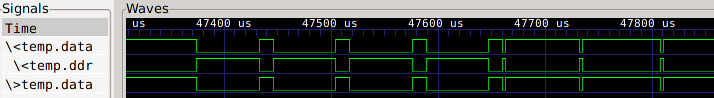
\includegraphics[width=\textwidth]{images/gtkwave}
\caption{GTKWave}
\label{fig:gtkwave}
\end{figure}


%%%%%%%%%%%%%%%%%%%%%%%%%%%%%%%%%%%%%%%%%%%%%%%%%%%%%%%%%%%%%%%%%%%%%%%%%%%%%%%%
\section{Example of an internal module implementation} %TODO
%%%%%%%%%%%%%%%%%%%%%%%%%%%%%%%%%%%%%%%%%%%%%%%%%%%%%%%%%%%%%%%%%%%%%%%%%%%%%%%%

%%%%%%%%%%%%%%%%%%%%%%%%%%%%%%%%%%%%%%%%%%%%%%%%%%%%%%%%%%%%%%%%%%%%%%%%%%%%%%%%
\section{Core Definitions}
%%%%%%%%%%%%%%%%%%%%%%%%%%%%%%%%%%%%%%%%%%%%%%%%%%%%%%%%%%%%%%%%%%%%%%%%%%%%%%%%

%%
%% = eof =====================================================================
%%
